\documentclass[tikz,border=2pt]{standalone}
\usetikzlibrary{calc}
\usetikzlibrary{intersections}
\usetikzlibrary{patterns}
\usepackage{bm}
\usetikzlibrary{positioning}
\usetikzlibrary{shapes}

\begin{document}

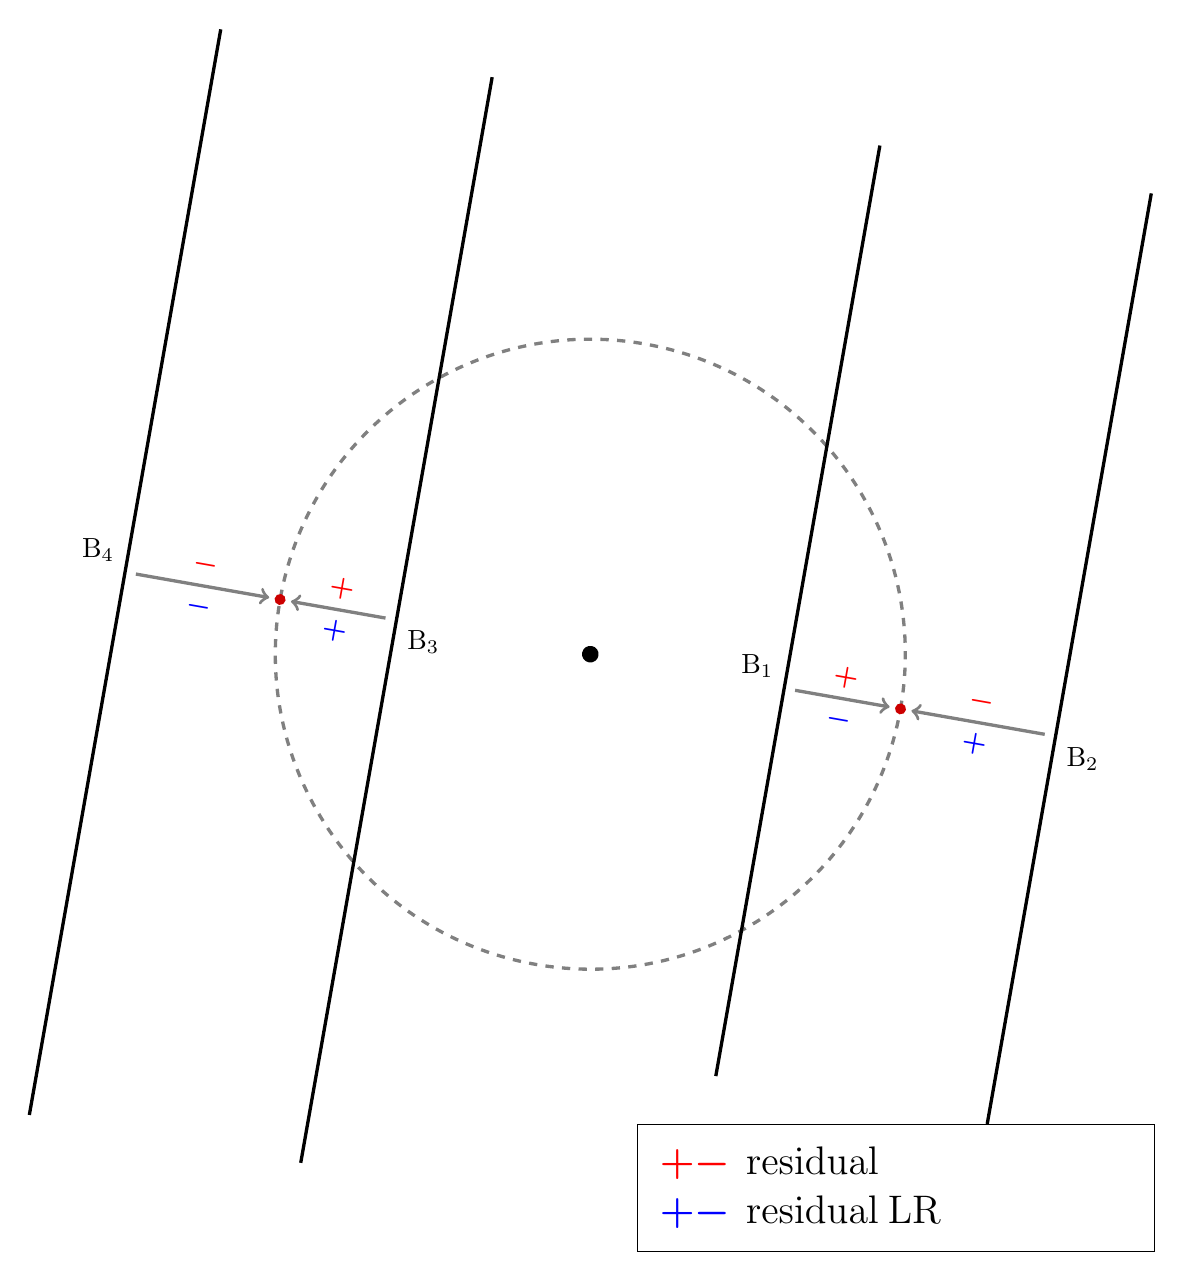
\begin{tikzpicture}[rotate=-10, very thick]
    
    % Draw wire
    \fill [black] (0,0) circle [radius=3pt]; %node [black, below] {A};
    \draw [name = measure, dashed, gray] (0,0) circle [radius=4];

    % Draw tracks
    \draw [name = track1] (2.5,-5) -- (2.5,7);
    \draw [name = track2] (6,-5) -- (6,7);
    \draw [name = track3] (-2.5,-7) -- (-2.5,7);
    \draw [name = track4] (-6,-7) -- (-6,7);

    % Draw points
    \coordinate (A) at (0,0);
    \coordinate (B1) at (2.5,0);
    \coordinate (B2) at (6,0);
    \coordinate (B3) at (-2.5,0);
    \coordinate (B4) at (-6,0);
    \coordinate (C12) at (4,0);
    \coordinate (C34) at (-4,0);
    
    \fill (B1) circle [radius=0pt] node [above left] at (B1) {B$_1$};
    \fill (B2) circle [radius=0pt] node [below right] at (B2) {B$_2$};
    \fill (B3) circle [radius=0pt] node [below right] at (B3) {B$_3$};
    \fill (B4) circle [radius=0pt] node [above left] at (B4) {B$_4$};
    \fill [red!80!black] (C12) circle [radius=2pt];% node [above left] at (C12) {C$_{12}$};
    \fill [red!80!black] (C34) circle [radius=2pt];% node [above left] at (C34) {C$_{34}$};

    % Draw arrow
    \draw [->, shorten >=4pt, shorten <=4pt, gray] (B1) -- (C12);
    \draw [->, shorten >=4pt, shorten <=4pt, gray] (B2) -- (C12);
    \draw [->, shorten >=4pt, shorten <=4pt, gray] (B4) -- (C34);
    \draw [->, shorten >=4pt, shorten <=4pt, gray] (B3) -- (C34);

    % Draw signs for residual
    \node [rotate=-10,above, red] at ($(B1)!0.5!(C12)$) {$\bm{+}$};
    \node [rotate=-10,above, red] at ($(B2)!0.5!(C12)$) {$\bm{-}$};
    \node [rotate=-10,above, red] at ($(B3)!0.5!(C34)$) {$\bm{+}$};
    \node [rotate=-10,above, red] at ($(B4)!0.5!(C34)$) {$\bm{-}$};
    % Draw signs for residual LR
    \node [rotate=-10,below, blue] at ($(B1)!0.5!(C12)$) {$\bm{-}$};
    \node [rotate=-10,below, blue] at ($(B2)!0.5!(C12)$) {$\bm{+}$};
    \node [rotate=-10,below, blue] at ($(B3)!0.5!(C34)$) {$\bm{+}$};
    \node [rotate=-10,below, blue] at ($(B4)!0.5!(C34)$) {$\bm{-}$};

    % Draw legend
    % \node [draw,align=left, text width=13.5cm, inner sep=8pt, line width=0.5pt] at (5,-6) { \Large
    %     {\color{red}  $\bm{+-}\,$} track being too close or too far to the wire\\
    %     {\color{blue} $\bm{+-}\,$} track being to the right or to the left of the measurement\\
    %     {\color{gray} $\longrightarrow\,\,$} direction for correction
    %     };

    \node [draw,align=left, text width=6cm, inner sep=8pt, line width=0.5pt] at (5,-6) { \Large
        {\color{red}  $\bm{+-}\,$} residual \\
        {\color{blue} $\bm{+-}\,$} residual LR\\
        };
    

\end{tikzpicture}


\end{document}